\chapter{提案}
本章では,SBCを用いたマルチディスプレイシステムにおけるOS仮想化技術を用いた仮想化と,コンテナ技術を用いたSBCマルチディスプレイシステムのフレーム処理並列化について設計・提案する.
本章では,まず3.1節でOS仮想化基盤とコンテナ技術について簡単に説明する.
そして,続く3.2節でOS仮想化基盤を利用したSBCマルチディスプレイシステムのコンテナ仮想化についての設計と実装について述べる.
3.3章では映像ベースのアプリケーションをコンテナ仮想化することによって生じる問題と,その解決法について述べる.
3.4章では,本研究の中心部分となるヘッドノード内でのフレーム処理の改良について,その設計指針を述べ,
具体的な実装について記す.

\section{OS仮想化基盤とコンテナ技術}
OS仮想化基盤には,代表的なものとしてDocker \cite{docker}が挙げられる.


\section{MDのコンテナ化}
以下,コンテナ技術を用いたSBCマルチディスプレイシステムの実装について書く

\section{コンテナを通したディスプレイの制御}
コンテナ内からディスプレイを制御する方法について書く
フレームバッファを利用したディスプレイ表示のメカニズムについて図を使って解説できると良い


\section{ヘッドノードでのフレーム処理の改良}
ヘッドノード内でのコンテナを用いたフレーム処理の並列化について書く
メインコンテナ,圧縮コンテナの実装や動作などについて図やフローチャートを用いて解説する

\subsection*{フレーム処理のコンテナ並列化}
\subsection*{コンテナ間でのフレーム受け渡し処理}
System V IPC \cite{kerrisk2010linux,linux_kernel}
\begin{figure}[H]
    \hspace*{\fill}
    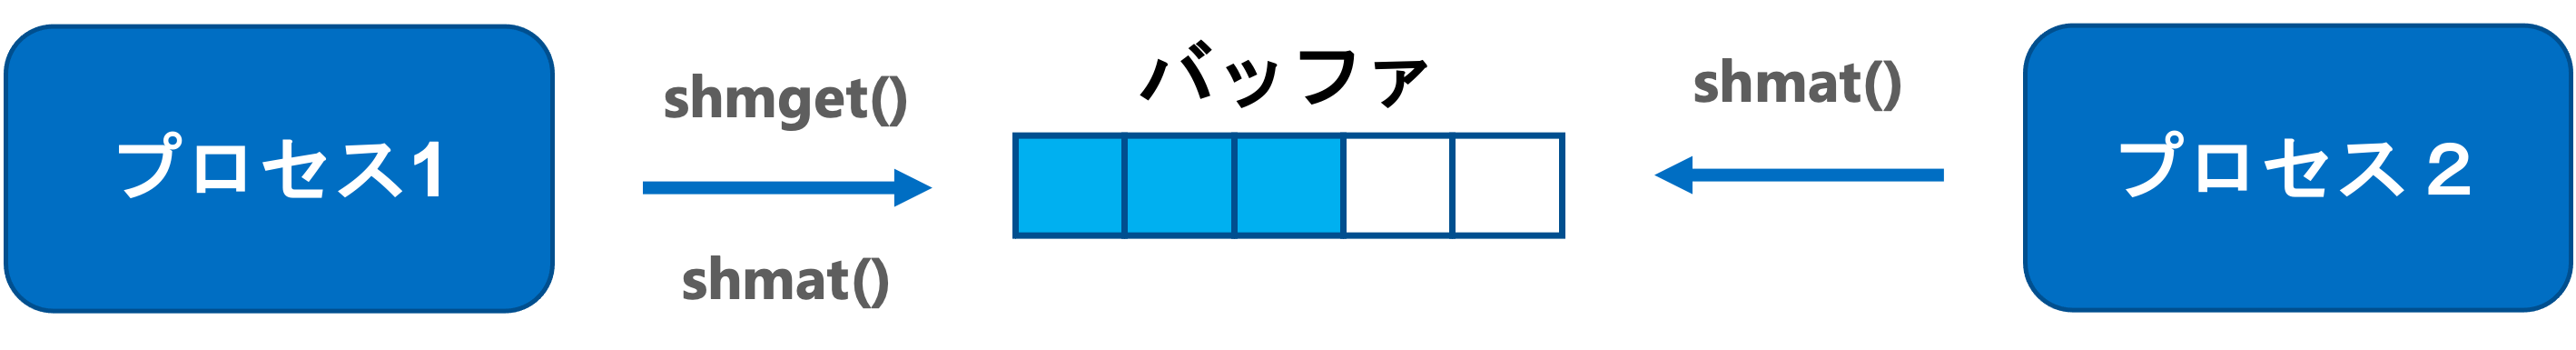
\includegraphics[width=\linewidth]{./fig/shared_memory.eps}
    \hspace*{\fill}
    \caption{共有メモリの使用例}
   \end{figure}

\begin{figure}[H]
    \hspace*{\fill}
    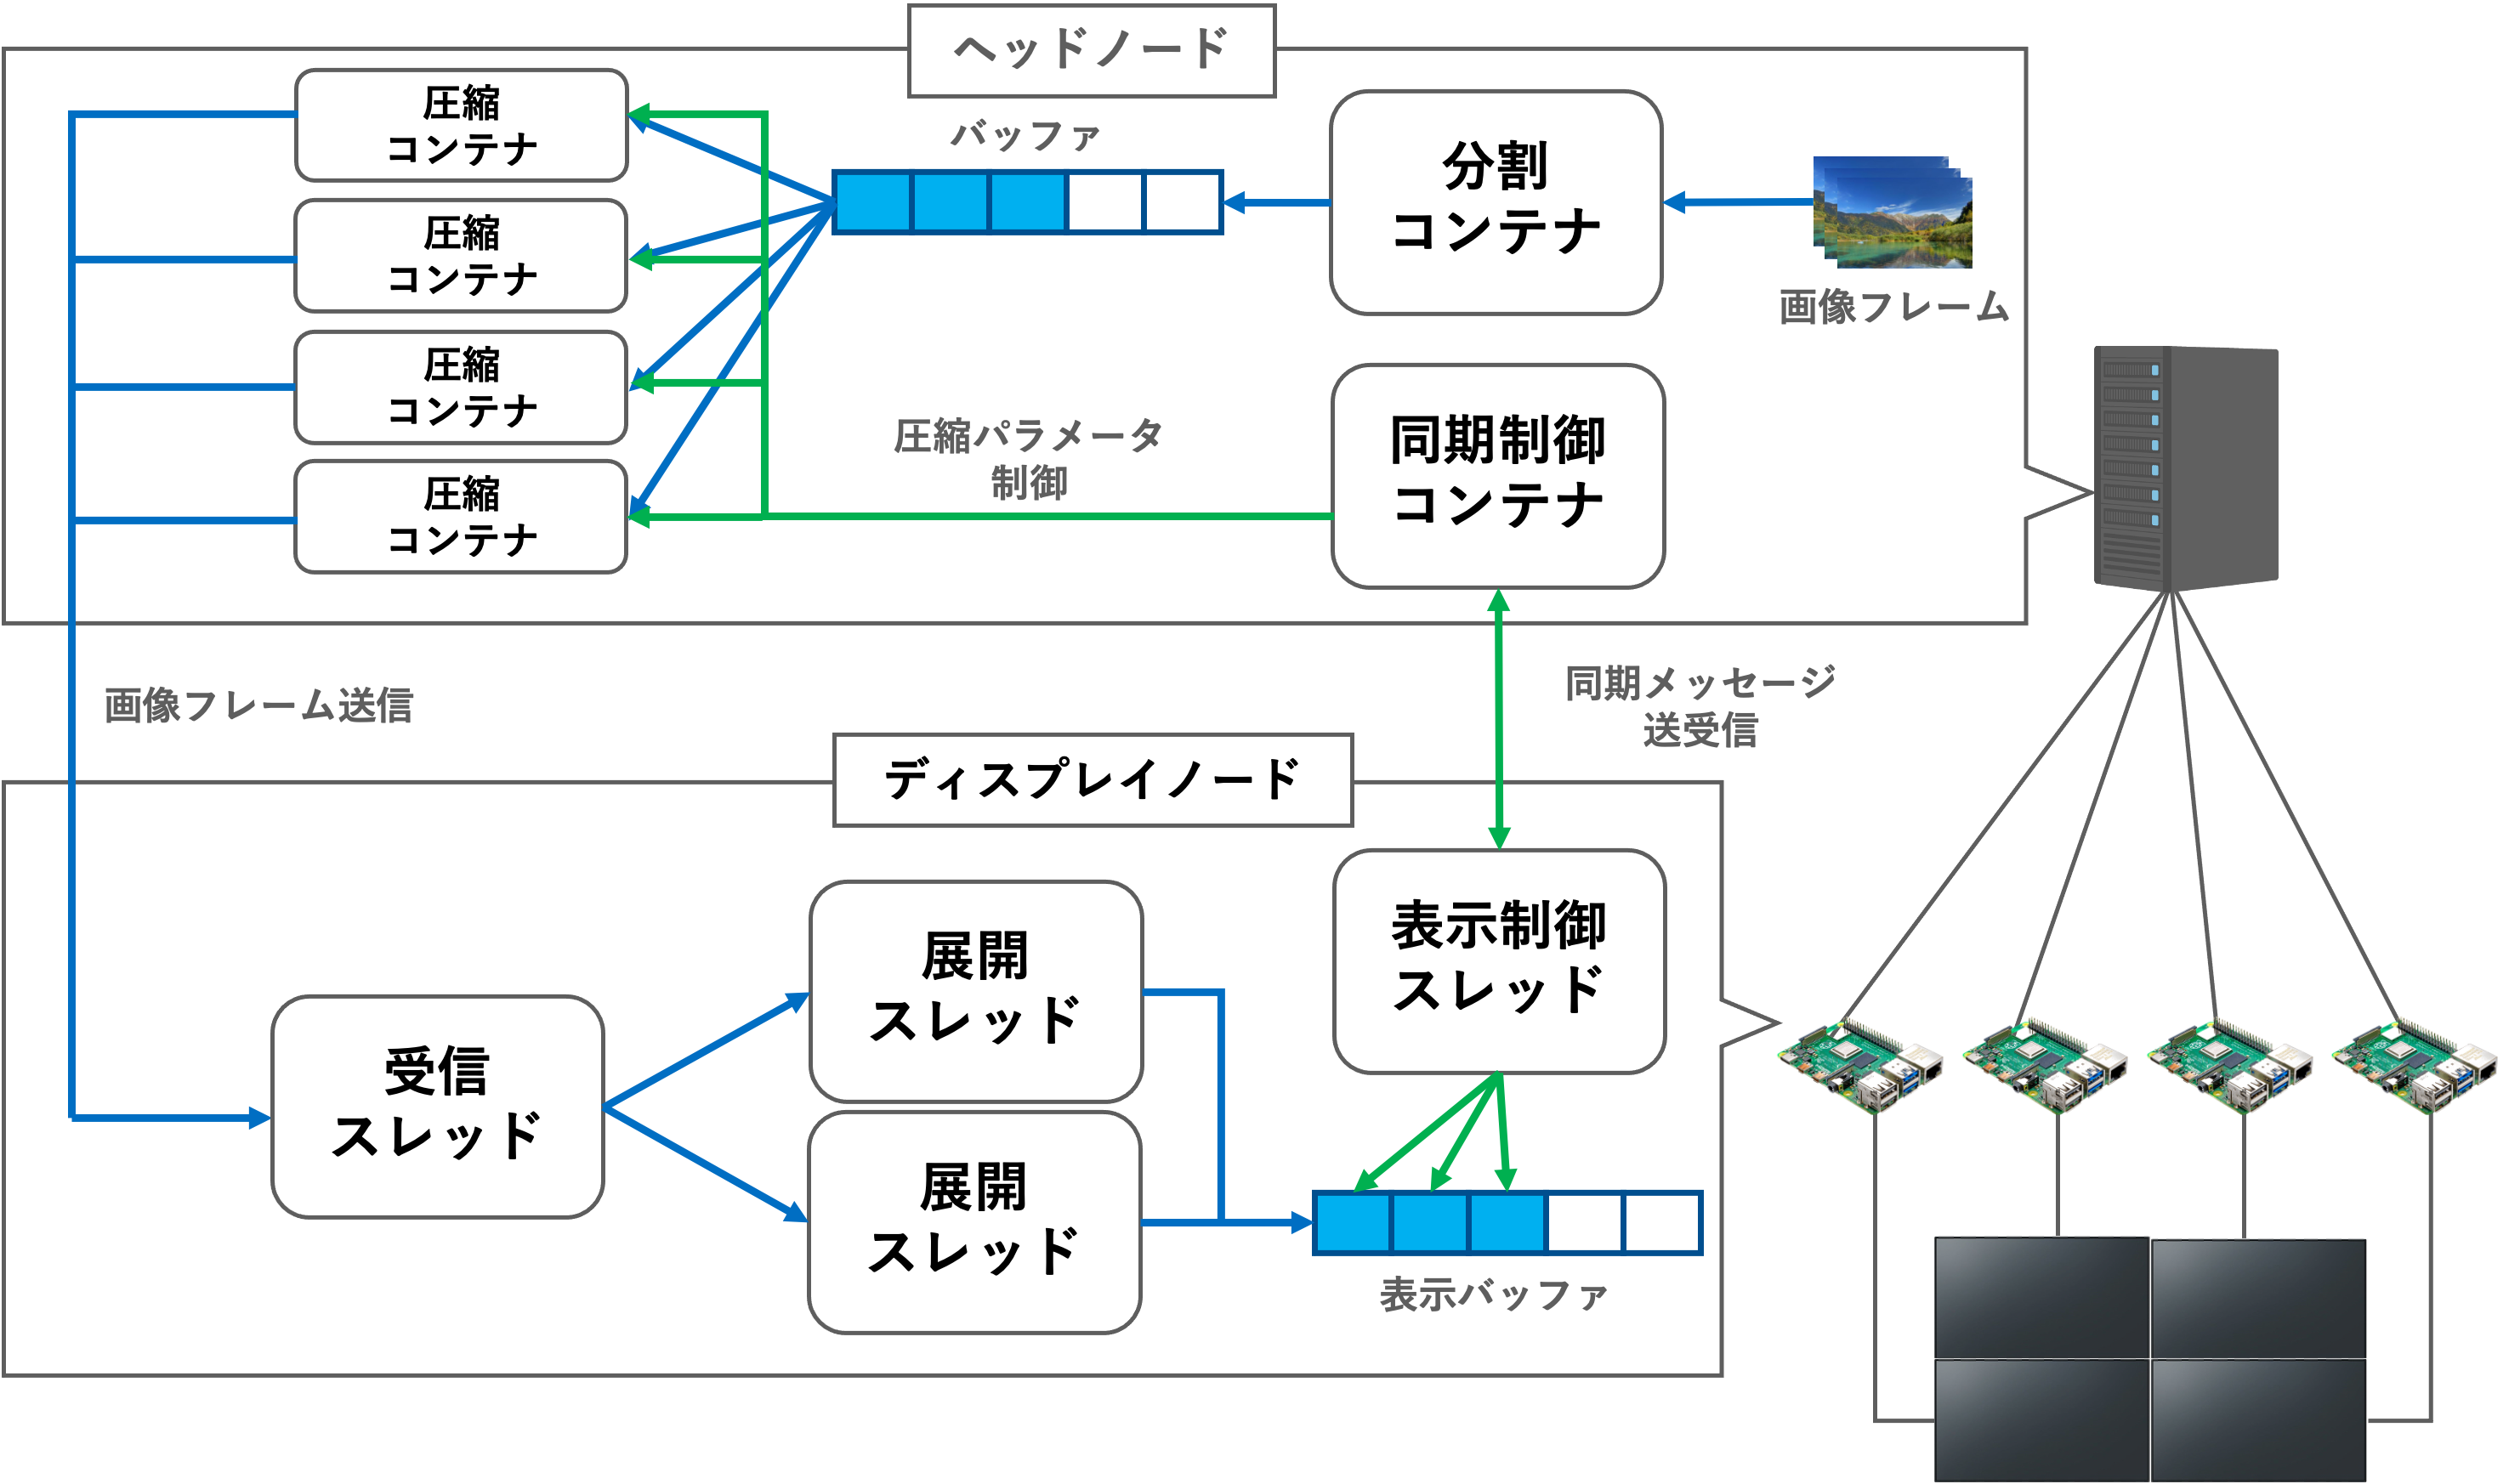
\includegraphics[width=\linewidth]{./fig/system_flow.eps}
    \hspace*{\fill}
    \caption{提案手法を用いたMDの動作フロー}
   \end{figure}
